\documentclass[conference]{IEEEtran}
\usepackage[utf8]{inputenc}
\usepackage[T1]{fontenc}
\usepackage{amsmath,amssymb}
\usepackage{booktabs}
\usepackage{graphicx}
\usepackage{cite}
\usepackage{url}
\usepackage{microtype}
\graphicspath{{figures/}}

% Live-replay numbers: generated by paper/make_replay_tex.py from results/replay3/
% generated by paper/make_replay_tex.py -- do not edit
\newcommand{\ReplayAbstract}{On a real cluster it resizes pods in place without restarts; a trace replay against the HPA with 3 seeds is mixed: it dominated an HPA setting on 2 of 3 seeds and was dominated on 0.}
\newcommand{\ReplayBody}{An open-loop load generator replayed a 24-minute demand trace (12 minutes of an Azure trace, then a flash crowd to five times the mean) against a CPU-bound service costing 61\,ms of CPU per request, with a 0.3\,s latency objective (five times the service time, as in the simulator). Each controller started from the same allocation with three unscored lead-in minutes, and both sides could reach the same ten cores. We ran the HPA at three utilisation targets, to give it a cost frontier, and CHIMERA at its evaluated default, with 3 seeds each (Table~\ref{tab:replay}).

\begin{table}[t]
\caption{Live replay, mean of 3 seeds. Viol.\ = requests over 0.3\,s (\%), with the range over seeds; $>$1\,s = requests over one second (\%); CPU in core-minutes.}
\label{tab:replay}
\centering
\begin{tabular}{@{}lrrrr@{}}
\toprule
Controller & Viol. & Range & $>$1\,s & CPU \\
\midrule
HPA, 70\,\% target & 48.9 & 44.1--55.2 & 39.3 & 85.3 \\
HPA, 50\,\% target & 23.5 & 21.9--26.4 & 14.9 & 102.4 \\
HPA, 35\,\% target & 16.3 & 11.2--22.5 & 5.4 & 124.3 \\
CHIMERA & 32.1 & 26.2--43.1 & 20.9 & 80.9 \\
\bottomrule
\end{tabular}
\end{table}

On 2 of 3 seeds CHIMERA dominated at least one HPA setting: it used no more CPU and had fewer violations. Where CHIMERA's cost lay inside the range the HPA settings span (1 of 3 seeds), interpolating the HPA's violation rate at that cost gave CHIMERA fewer violations on 0 of 1, with a mean gap of -1.9 points. On average CHIMERA used 80.9 core-minutes for 32.1\,\% violations; the HPA needed 85.3 for 48.9\,\% at a 70\,\% target, 102.4 for 23.5\,\% at 50\,\%, and 124.3 for 16.3\,\% at 35\,\%. With 3 seeds no significance test is meaningful, and we treat this as indicative. Every controller missed the objective far more often than in simulation: a 61\,ms request on a pod limited to half a core exceeds a single CFS quota period, so the simulator's latency law is kinder than this service. In an earlier single-run comparison a request-rate signal reached a given allocation 20 to 25\,s sooner after the spike began than the default one-minute CPU-usage rate.}
\newcommand{\ReplayConclusion}{On a real cluster the operator works, and a small trace-replay experiment is mixed: it dominated an HPA setting on 2 of 3 seeds and was dominated on 0. A larger live study, with more seeds and a service whose latency the simulator models faithfully, is the main work that remains.}


\begin{document}

\title{CHIMERA: Joint Horizontal and Vertical Pod Autoscaling\\with a Fast and a Slow Actuator}

% Affiliations and e-mail addresses: add an \IEEEauthorblockA{...} under the names.
\author{\IEEEauthorblockN{Adithyan C S S, Ajay M, and Rohith Pranov V}}

\maketitle

\begin{abstract}
Kubernetes can now change the CPU of a running pod in well under a second, while a new
replica still takes tens of seconds to serve. Existing autoscalers use one of these
actuators or run a separate loop for each. We present CHIMERA, a controller that plans
replica count and CPU per pod together. It combines a linear-quadratic regulator whose
state includes the replicas that have been ordered but are not yet serving, a cascade in
which a five-second inner loop owns CPU and a fifteen-second outer loop owns replicas, and
a capacity rule that prices the risk of missing a latency objective against the cost of
CPU over conformal demand scenarios. Design choices were made on a development split and
judged on data they did not see. In simulation, at equal CPU cost, CHIMERA has fewer
objective violations than HPA, VPA, their combination, AAPA, a MagicScaler-style scaler
and KOSMOS on 47 of 48 trace-by-baseline comparisons on a held-out set, and on all 117 on
twenty real traces that no design step used: ten production serverless functions and ten
web-server windows. The advantage persists, with a smaller margin, under latency laws the
controller does not assume. An ablation shows that fast release of CPU, joint control and
single ownership of each actuator carry the benefit, that a coupling penalty and a
Lyapunov filter from the original design change no decision, and that the risk-priced
capacity rule helps only when its latency model is roughly right. A Kubernetes operator
runs the same control law. \ReplayAbstract
\end{abstract}

\begin{IEEEkeywords}
autoscaling, Kubernetes, in-place pod resize, serverless, optimal control, conformal prediction
\end{IEEEkeywords}

\section{Introduction}

A service on Kubernetes can be given more capacity in two ways: more pod replicas, or more
CPU per pod. The two actuators differ by two orders of magnitude in speed. A new replica
typically needs tens of seconds to be scheduled, started and made ready. Since in-place pod
resize~\cite{kep1287} (on by default from Kubernetes~1.33, stable in~1.35) the CPU of a
running pod can be changed in well under a second without restarting the container.

The stock autoscalers do not exploit this. The Horizontal Pod Autoscaler (HPA) changes the
replica count from average utilisation; the Vertical Pod Autoscaler (VPA) changes pod size
from usage history. Run together on the same CPU signal they interfere, and neither models
the fact that a replica it has just ordered is not serving yet. Predictive horizontal
scalers such as AAPA~\cite{aapa} and MagicScaler~\cite{magicscaler} handle uncertainty but
have only the slow actuator, so they must pay for forecast error with standing headroom.
Systems that do use both actuators, such as KOSMOS~\cite{kosmos}, run two separately
designed loops.

This paper asks how one controller should use a slow and a fast actuator on the same
resource to hold a per-request latency objective at the lowest CPU cost. We present
CHIMERA, which combines three ideas.

\emph{A delay-aware joint control law.} Replicas and CPU per pod are driven by one
linear-quadratic regulator whose state includes the replicas that have been ordered but
are not yet serving, so the same capacity is never ordered twice.

\emph{A cascade that gives each actuator one owner.} A 5\,s inner loop owns CPU: it raises
CPU as soon as a surge is statistically visible and returns it shortly after the surge
passes. A 15\,s outer loop owns replicas and changes them only when CPU resizing cannot
absorb the change.

\emph{Risk-priced capacity.} The amount of capacity is chosen by minimising expected
violations of the objective plus a price per core, over demand scenarios drawn from
conformal forecast errors.

We do not claim to be the first to resize in place before scaling out (Themis~\cite{themis}
does so for inference serving), to optimise both axes jointly (Ship et al.~\cite{ship}
pose it as a fluid optimal-control problem), to trade cost against violation risk
(MagicScaler), or to use conformal calibration in an autoscaler (BACC~\cite{bacc}, for the
horizontal axis). Our contributions are:
\begin{itemize}
\item the combination above for a sub-second and a tens-of-seconds actuator, with an
explicit model of replicas in flight (Section~\ref{sec:design});
\item an evaluation protocol that separates design data from verdict data and compares
controllers at equal cost (Section~\ref{sec:method});
\item results on a held-out set, on twenty real traces no design step used, and under
latency laws the controller does not assume (Sections~\ref{sec:heldout}
and~\ref{sec:general});
\item an account of which parts of the design carry the benefit, including two mechanisms
that turned out to change no decision and one that helps only under its own assumptions;
\item a Kubernetes operator, validated on Kubernetes~1.33 and compared with the HPA by
trace replay (Section~\ref{sec:live}).
\end{itemize}

\section{Background and Related Work}

\textbf{In-place resize.} KEP-1287~\cite{kep1287} lets the kubelet change a running
container's CPU and memory through the \texttt{pods/resize} subresource. For CPU this is a
cgroup update and takes effect without a restart. Hsieh and Chou~\cite{hsieh} study the
feature for serverless cold starts; Sponge~\cite{sponge} uses it to follow changing
objectives in inference serving.

\textbf{Joint horizontal and vertical scaling.} Autopilot~\cite{autopilot} scales both
axes at Google from usage history, with slack and out-of-memory rate as objectives.
SHOWAR~\cite{showar} sizes pods from the variance of historical usage and scales replicas
with a controller on kernel metrics. KOSMOS~\cite{kosmos}, the closest system to ours,
resizes containers with control-theoretic planners on response time and adds or removes
replicas with a heuristic controller. Themis~\cite{themis} absorbs a surge with in-place
vertical scaling and moves to horizontal scaling once the workload settles; it chooses
configurations by dynamic programming over profiled latency, forecasts with an LSTM
without prediction intervals, and handles replica start-up through its transition
procedure, not through a model of replicas in flight. Ship et al.~\cite{ship} derive
resources per replica and replica counts from a fluid approximation of a queueing network
solved as a separated continuous linear program; their model has no replica start-up delay
and takes demand rates as given. Autothrottle~\cite{autothrottle} uses a bi-level
structure for CPU alone: a learned application-level controller sets throttle targets that
per-service controllers meet. CHIMERA differs from these in planning both actuators from
one target with an explicit state for in-flight replicas, in closing the loop every five
seconds, and in sizing capacity by priced risk.

\textbf{Predictive and uncertainty-aware scaling.} MagicScaler~\cite{magicscaler} forecasts
demand with a multi-scale attentive Gaussian process and chooses the number of instances
with a loss that trades running cost against the risk of violating quality of service;
this is the nearest precedent for our capacity rule. AAPA~\cite{aapa} classifies serverless
workloads into four archetypes and applies a target and cooldown per archetype, widened by
calibrated confidence. BACC~\cite{bacc} wraps a forecaster in adaptive conformal inference
and steers horizontal provisioning with a controller on a violation budget.
FIRM~\cite{firm} localises the microservice responsible for a violation and reprovisions
it. All of these act on one axis.

\section{Design}
\label{sec:design}

Fig.~\ref{fig:arch} gives the structure. Every 15\,s the outer loop runs the steps of
Sections~\ref{sec:forecast}--\ref{sec:lqr}; every 5\,s the inner loop runs
Section~\ref{sec:inner}.

\begin{figure}[t]
\centering
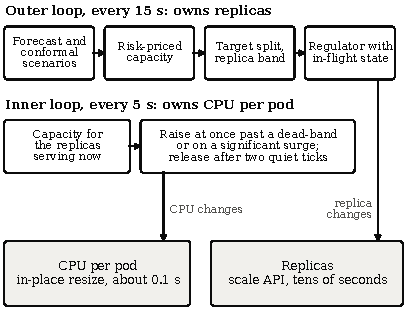
\includegraphics[width=\columnwidth]{fig_architecture.pdf}
\caption{The two loops and the actuator each owns.}
\label{fig:arch}
\end{figure}

\subsection{Forecast}
\label{sec:forecast}

A gradient-boosted quantile model, conformalised on a held-back window~\cite{cqr}, gives a
90\,\% interval for next-minute demand. Because a learned model has nothing to say about a
regime it has not seen, a second, model-free margin is kept beside it: the last observed
value plus a split-conformal quantile of recent one-step changes. An ADWIN
detector~\cite{adwin} on the forecast error discards that margin's history when the regime
changes. The operator, which has no training history for a newly attached service, uses the
model-free construction around an exponentially weighted mean.

\subsection{Risk-priced capacity}
\label{sec:risk}

Let $u$ be utilisation and suppose a request misses the latency objective with probability
$p(u)=\exp(-k(1-u))$ below saturation, where $k$ is the ratio of the objective to the mean
service time, estimated online. Given demand scenarios $L_1,\dots,L_n$ (the current load,
the current load plus each recent signed one-step change, and the forecast upper bound),
total capacity is
\begin{equation}
c^\ast=\arg\min_c\ \frac{1}{n}\sum_{i=1}^{n} L_i\,p\!\left(\frac{L_i}{c}\right)+\lambda c,
\qquad \lambda=p'(u_0)\,u_0^2 .
\label{eq:risk}
\end{equation}
The price $\lambda$ is fixed by one knob $u_0$: with it, a demand known with certainty
gives $c^\ast=L/u_0$, so $u_0$ reads as an ordinary target utilisation. Under uncertainty
the convexity of $p$ decides how much headroom is worth buying. The objective is not convex
(violation probability saturates near full utilisation), so it is minimised on a grid and
refined, over capacities that keep the expected load below saturation.

\subsection{Target split and replica band}

Capacity is split into a target $x^\ast=[v^\ast,h^\ast]$ (CPU per pod, replicas) with
$h^\ast v_{\max}\ge c^\ast$. Between $\lceil c^\ast/(0.85\,v_{\max})\rceil$ and
$\lfloor c^\ast/v_{\min}\rfloor$ replicas, any replica count can carry $c^\ast$ by resizing
CPU alone, while every added replica spends its boot time allocated but not serving. Inside
this band $h^\ast$ is left at the current count. $v^\ast$ is sized for the replicas that
are serving now, so the fast actuator covers the gap while ordered replicas boot and hands
the capacity back as they arrive.

\subsection{Delay-augmented regulator}
\label{sec:lqr}

The tracking error is augmented with the replicas in flight:
\begin{equation}
e=\bigl[\,v-v^\ast,\ h_{\mathrm{serving}}-h^\ast,\ \Delta h_{t-1},\dots,\Delta h_{t-d}\,\bigr]^{\top},
\quad u=-Ke,
\end{equation}
with $K$ from the discrete algebraic Riccati equation for $Q=\mathrm{diag}(30,10)$ and
$R=\mathrm{diag}(0.05,1)$, and $d=\lfloor\tau/\Delta t\rfloor$ slots for a boot time $\tau$
and control period $\Delta t$ (one slot for 20\,s and 15\,s). Only scale-ups enter the
buffer; a removed replica stops serving at once. The action is clipped to the resource
bounds and a total capacity budget. Closed-loop stability follows from the Riccati solution
$P$: $V=e^{\top}Pe$ decreases along $u=-Ke$.

On a real cluster boot time is not a constant. The operator therefore reconciles the buffer
with what the cluster reports, taking the replicas in flight to be the desired count minus
the ready count, before each step (Section~\ref{sec:live} describes the failure this
prevents).

\subsection{Inner loop}
\label{sec:inner}

Between outer steps only CPU moves. Every 5\,s the inner loop recomputes the capacity of
Section~\ref{sec:risk} for the serving replicas. It raises CPU per pod at once if the need
exceeds the allocation by a relative dead-band (30\,\%), or if a Poisson test on a short
arrival window shows a significant surge, and lowers it once the need has stayed 15\,\%
below the allocation for two consecutive ticks. Acquiring CPU takes about 0.1\,s, so there
is no reason to hold it through a long cooldown. The dead-band bounds how often pods are
resized.

\subsection{Implementation}

The controller is about 350 lines of Python; one control step takes about 0.3\,ms. The
Kubernetes operator watches a custom resource, reads CPU usage and optionally request rate
from Prometheus, resizes CPU through \texttt{pods/resize}, changes replicas through the
Deployment scale subresource, and writes its decision to the resource's status.

\section{Evaluation Method}
\label{sec:method}

\subsection{Simulator}

We extend the discrete-event simulator released with AAPA~\cite{aapa} to two dimensions:
pods have a CPU size, a replica takes 20\,s to boot, and an in-place resize takes 0.1\,s.
Requests have exponentially distributed CPU service times with mean 0.1\,s and are slowed
by a factor $1/(1-u)$ at utilisation $u$; the latency objective is 0.5\,s.
Section~\ref{sec:robust} replaces both the distribution and the slowdown law.

\subsection{Workloads and splits}

Table~\ref{tab:sets} lists the trace sets. Every design choice was made on the dev set.
All sets use an unscored 20-minute warm-up so that no controller is scored on its cold
start. The Azure excerpts appear in both the dev and the held-out set, in different
windows; the two external sets exist to remove that dependence. Their functions and windows
were fixed by rule before any controller ran on them. Request rates are rescaled so that
the busiest minute of a window fits what the horizontal-only baselines can serve at their
replica limit.

\begin{table}[t]
\caption{Trace sets. Each trace is 100 minutes; minutes 70--100 are scored.}
\label{tab:sets}
\centering
\begin{tabular}{@{}lp{4.4cm}l@{}}
\toprule
Set & Traces & Role \\
\midrule
Dev & 5 Azure Functions 2019 excerpts~\cite{shahrad} (minutes 40--70), 4 synthetic shapes; 3 seeds & design \\
Held-out & the same 5 Azure excerpts (minutes 70--100), 4 other synthetic shapes; 10 new seeds & verdict \\
Serverless & 10 production functions, Huawei private cloud 2023~\cite{huawei} & verdict \\
Web & 6 NASA and 4 ClarkNet web-server windows, 1995~\cite{ita} & verdict \\
\bottomrule
\end{tabular}
\end{table}

\subsection{Baselines}

HPA; VPA with five fixed replicas; HPA and VPA together; AAPA~\cite{aapa}; a scaler in the
style of MagicScaler~\cite{magicscaler} (our implementation of the idea, not the authors'
predictor or code); and KOSMOS~\cite{kosmos}, reimplemented from the paper with its gains
tuned on the dev set. Every controller has the same resource bounds and starts from the
same allocation.

\subsection{Comparison at equal CPU}

Controllers at their default settings sit at different points of the cost--violation
trade-off, so a lower violation rate may only mean more CPU was spent. Every controller is
therefore swept over its own conservatism setting (target utilisation; for KOSMOS its
response-time setpoint), and each baseline's violation rate is interpolated on its own
frontier at CHIMERA's CPU cost, trace by trace, wherever the two cost ranges overlap.
Significance is tested on one gap per trace and seed (the same request stream) with a
one-sample Wilcoxon signed-rank test, Holm-corrected across baselines.

\section{Results on the Held-Out Set}
\label{sec:heldout}

The main comparison is 3{,}870 runs (43 configurations, 9 traces, 10 seeds); the frontier
sweep is 4{,}095 runs (5 seeds).

\subsection{Equal CPU}

Table~\ref{tab:heldout} gives, for each baseline, the number of traces on which CHIMERA has
fewer violations at the same CPU cost and the mean difference. Counting per-trace frontier
comparisons, CHIMERA wins 47 of 48. The exception is the MagicScaler-style scaler on one
Azure trace (a high, flat, noisy load), by 0.66 points. VPA is compared on fewer traces
because its cost range, fixed by its five replicas, does not always overlap CHIMERA's.

\begin{table}[t]
\caption{Held-out set at equal CPU. Gap = baseline minus CHIMERA, in percentage points of
violation rate. All $p<0.001$ (Wilcoxon, Holm).}
\label{tab:heldout}
\centering
\begin{tabular}{@{}lrrrr@{}}
\toprule
 & \multicolumn{2}{c}{Azure} & \multicolumn{2}{c}{Synthetic} \\
\cmidrule(lr){2-3}\cmidrule(l){4-5}
Baseline & won & gap & won & gap \\
\midrule
AAPA & 5/5 & $+1.68$ & 4/4 & $+5.28$ \\
HPA & 5/5 & $+4.71$ & 4/4 & $+8.04$ \\
HPA+VPA & 5/5 & $+4.26$ & 4/4 & $+6.27$ \\
KOSMOS & 5/5 & $+5.65$ & 4/4 & $+6.00$ \\
MagicScaler-style & 4/5 & $+4.72$ & 4/4 & $+7.31$ \\
VPA & 3/3 & $+2.81$ & 3/3 & $+9.69$ \\
\bottomrule
\end{tabular}
\end{table}

\subsection{Default settings}

Table~\ref{tab:default} shows each controller at its default setting. Against AAPA on the
Azure traces CHIMERA has 0.99 points fewer violations ($p=0.003$) for a CPU difference of
$+14.7$ core-minutes that is not significant ($p=0.086$); on the synthetic shapes it has
1.39 points fewer violations with 30\,\% less CPU. Two things in the table do not favour
CHIMERA. KOSMOS has fewer violations on the synthetic shapes (3.42\,\% against 5.63\,\%) at
1.8 times the CPU; the equal-CPU comparison is what separates them. And CHIMERA has the
lower seed-mean violation rate than AAPA on only 3 of the 5 Azure traces.

\begin{table}[t]
\caption{Held-out set, default settings. Viol.\ = share of requests over the objective;
CPU in core-minutes per 30-minute run; Act.\ = scaling actions per run.}
\label{tab:default}
\centering
\setlength{\tabcolsep}{3.5pt}
\begin{tabular}{@{}lrrrrr@{}}
\toprule
 & \multicolumn{2}{c}{Azure} & \multicolumn{2}{c}{Synthetic} & \\
\cmidrule(lr){2-3}\cmidrule(lr){4-5}
Controller & Viol. & CPU & Viol. & CPU & Act. \\
\midrule
CHIMERA & 5.93\,\% & 251.5 & 5.63\,\% & 71.8 & 32.5 \\
AAPA & 6.92\,\% & 236.8 & 7.02\,\% & 101.9 & 6.7 \\
KOSMOS & 8.71\,\% & 326.7 & 3.42\,\% & 132.1 & 274.8 \\
HPA+VPA & 14.06\,\% & 194.8 & 13.29\,\% & 65.2 & 19.2 \\
HPA & 15.60\,\% & 190.8 & 15.13\,\% & 63.7 & 14.5 \\
MagicScaler-style & 16.78\,\% & 181.1 & 14.41\,\% & 63.2 & 16.1 \\
VPA & 19.40\,\% & 169.2 & 15.16\,\% & 78.7 & 10.8 \\
\bottomrule
\end{tabular}
\end{table}

\subsection{Where the benefit comes from}

Table~\ref{tab:ablation} removes or re-adds one mechanism at a time. Rows are single
operating points: a row with fewer violations and more CPU is a different point on the
trade-off, not a better controller. Read that way, fast release is the largest effect:
without it CPU nearly doubles on the Azure traces and is 2.6 times higher on the synthetic
shapes. Joint control saves 7\,\% CPU on the Azure traces and 37\,\% on the synthetic
shapes against horizontal-only control, with 0.5 pod changes per run instead of 12. Single
ownership of CPU and the dead-band each remove more than half of the resizes that would
otherwise occur, and the replica band cuts pod changes from 8.6 to 0.5 per run.

The last three rows are negative results. The design began with a penalty on opposing
moves of the two actuators and a Lyapunov filter on the action; re-adding either, or a
guardrail against scaling in while replicas boot, leaves every one of the 90 runs
identical. Once each actuator has a single owner and replicas move rarely, opposing moves
do not arise, and the filter enforces a decrease the regulator already guarantees. The
reported controller does not run them.

Without in-place resize (a CPU change then needs a rolling restart) CHIMERA's violation
rate on the synthetic shapes rises from 5.63\,\% to 7.91\,\%: the design depends on the
fast actuator.

\begin{table}[t]
\caption{Ablation on the held-out set. Rs.\ = in-place resizes per run; Pods = replica
changes per run.}
\label{tab:ablation}
\centering
\setlength{\tabcolsep}{3pt}
\begin{tabular}{@{}lrrrrrr@{}}
\toprule
 & \multicolumn{2}{c}{Azure} & \multicolumn{2}{c}{Synthetic} & & \\
\cmidrule(lr){2-3}\cmidrule(lr){4-5}
Variant & Viol. & CPU & Viol. & CPU & Rs. & Pods \\
\midrule
Full controller & 5.93 & 251.5 & 5.63 & 71.8 & 32.5 & 0.5 \\
w/o fast release & 2.24 & 480.1 & 2.44 & 185.6 & 1.0 & 0.5 \\
horizontal only & 4.80 & 271.7 & 3.75 & 114.8 & 12.0 & 12.0 \\
w/o inner loop & 4.92 & 274.6 & 5.01 & 81.2 & 37.2 & 0.4 \\
CPU not single-owned & 5.12 & 267.4 & 4.90 & 75.7 & 79.7 & 0.5 \\
w/o dead-band & 4.96 & 269.1 & 4.80 & 75.8 & 84.1 & 0.5 \\
w/o replica band & 5.88 & 256.2 & 5.61 & 74.3 & 43.3 & 8.6 \\
w/o CQR & 6.21 & 242.6 & 5.62 & 69.8 & 37.8 & 0.4 \\
\midrule
+ coupling penalty & 5.93 & 251.5 & 5.63 & 71.8 & 32.5 & 0.5 \\
+ Lyapunov filter & 5.93 & 251.5 & 5.63 & 71.8 & 32.5 & 0.5 \\
+ scale-in guardrail & 5.93 & 251.5 & 5.63 & 71.8 & 32.5 & 0.5 \\
\bottomrule
\end{tabular}
\end{table}

\section{Does the Result Generalise?}
\label{sec:general}

\subsection{Real traces no design step used}

The Azure excerpts are few and were visible, in an earlier window, during design. We
therefore ran the unchanged controllers on two further sets: ten production serverless
functions from the Huawei private-cloud trace~\cite{huawei}, and ten windows of the NASA
and ClarkNet web-server logs~\cite{ita} (900 main runs and 3{,}150 sweep runs each).
Table~\ref{tab:external} and Fig.~\ref{fig:frontiers} give the results.

\begin{table}[t]
\caption{Twenty external real traces at equal CPU. Gap in percentage points; all
$p<0.001$.}
\label{tab:external}
\centering
\begin{tabular}{@{}lrrrr@{}}
\toprule
 & \multicolumn{2}{c}{Serverless} & \multicolumn{2}{c}{Web} \\
\cmidrule(lr){2-3}\cmidrule(l){4-5}
Baseline & won & gap & won & gap \\
\midrule
AAPA & 10/10 & $+2.02$ & 10/10 & $+2.00$ \\
HPA & 10/10 & $+3.99$ & 10/10 & $+4.53$ \\
HPA+VPA & 10/10 & $+2.72$ & 10/10 & $+3.89$ \\
KOSMOS & 10/10 & $+2.38$ & 10/10 & $+1.27$ \\
MagicScaler-style & 10/10 & $+4.37$ & 10/10 & $+4.66$ \\
VPA & 9/9 & $+1.77$ & 10/10 & $+2.20$ \\
\bottomrule
\end{tabular}
\end{table}

\begin{figure*}[t]
\centering
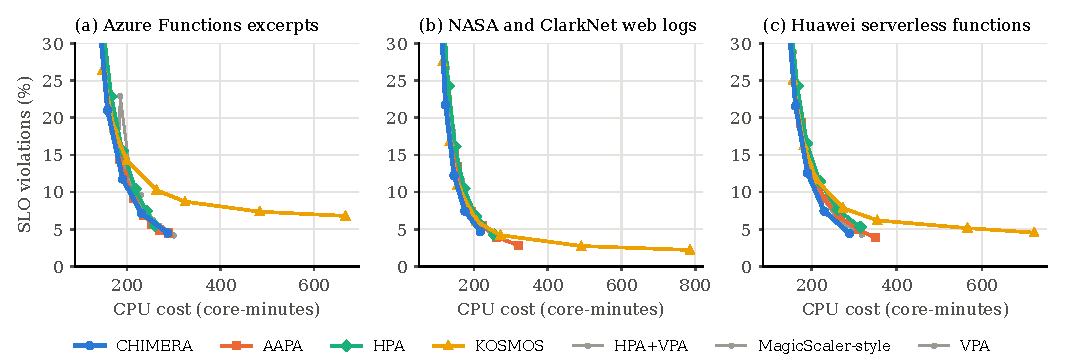
\includegraphics[width=\textwidth]{fig_frontiers.pdf}
\caption{Cost--violation frontiers on the three verdict sets. Each line sweeps one
controller over its conservatism setting; down and to the left is better.}
\label{fig:frontiers}
\end{figure*}

CHIMERA wins all 117 per-trace frontier comparisons (57 serverless, 60 web). At default
settings on the serverless traces it has 6.06\,\% violations at 251 core-minutes against
AAPA's 9.18\,\% at 230; on the web traces 6.18\,\% at 190 against 7.45\,\% at 194. KOSMOS
is the closest competitor. At its default setting it matches CHIMERA on the serverless
traces (6.16\,\%) and beats it on the web traces (4.22\,\%), for 45\,\% and 43\,\% more CPU
and about ten times as many resizes.

A first version of the web experiment scaled the request rates too high: the
horizontal-only baselines sat at their replica limit on every ClarkNet window and CHIMERA
``won'' 56 of 58 comparisons for the wrong reason. We discarded it, rescaled so that the
busiest minute fits the baselines' limit, and report only the re-run.

\subsection{A latency model the controller does not assume}
\label{sec:robust}

The capacity rule~\eqref{eq:risk} assumes the same latency law the simulator generates. To
test whether the result depends on that match, we re-ran the held-out sweep under three
other service-time distributions (lognormal, gamma, bimodal; same mean) and two other
slowdown laws, without re-tuning anything (Fig.~\ref{fig:robust}; this experiment used the
previous 10\,\% dead-band, which Table~\ref{tab:ablation} shows moves the frontier little).

\begin{figure}[t]
\centering
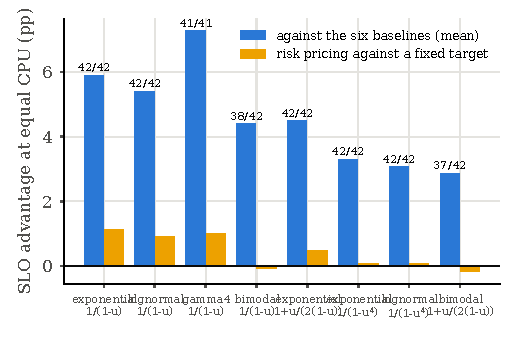
\includegraphics[width=\columnwidth]{fig_robustness.pdf}
\caption{Mean advantage at equal CPU under eight latency models. Bar labels give the
comparisons won out of those possible. Service times: exponential, lognormal, gamma,
bimodal. Slowdown laws: A $=1/(1-u)$, B $=1+u/(2(1-u))$, C $=1/(1-u^4)$. The first model is
the one the controller assumes.}
\label{fig:robust}
\end{figure}

The advantage over the baselines survives in every scenario, on every trace in six of
eight, with a mean gap between 2.9 and 7.3 points. With bimodal service times CHIMERA loses
to AAPA at equal CPU on four traces, by 0.1 to 0.7 points. The second series isolates the
capacity rule by comparing the controller with and without it: it is worth about one point
while the slowdown law matches its assumption, nothing under a hockey-stick law, and
slightly less than nothing with bimodal service times. On the external traces it is worth
0.2 points. The structural parts of the design carry the robust part of the result; the
capacity rule is a refinement that needs its latency model to be roughly right.

\section{On a Real Cluster}
\label{sec:live}

\subsection{Functional validation, and what it found}

On Kubernetes~1.33 (a local kind cluster, and one cloud instance running k3s) the operator
raised the CPU of running pods in place under load with no container restart, added a
replica once CPU alone could not cover the need, returned CPU when the new replica was
serving, and released everything when the load stopped.

The first run also removed a replica 15\,s after adding it. The controller's in-flight
buffer assumed the configured boot time of 20\,s; the real pod was ready within one control
period, so it was counted both as serving and as in flight. The simulator, whose boot time
is a constant, could not show this. The operator now reconciles the buffer with the cluster
before each step. Later runs exposed four further operator faults of the same kind (sizing
below observed demand on a cold start, a rate-based demand estimate below measured CPU, a
configured cost per request overwritten by online learning, and scale-in directly after
scale-out); each is fixed and covered by a regression test. We report this because it is
the reason to run on a cluster at all: it tests the assumptions the simulator bakes in.

\subsection{Trace replay against the HPA}

\ReplayBody

\begin{figure}[t]
\centering
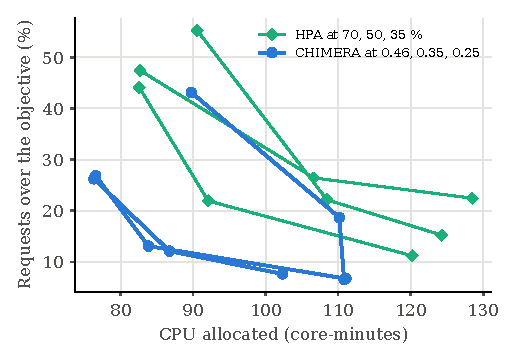
\includegraphics[width=\columnwidth]{fig_replay.pdf}
\caption{Live replay: share of requests over the objective against CPU allocated. One
line per seed joins the settings of each controller; down and to the left is better.}
\label{fig:replay}
\end{figure}

\section{Discussion and Limitations}

\textbf{What carries the result.} The fast actuator and single ownership. Returning CPU
within two ticks of a surge passing, instead of holding it through a cooldown, accounts
for about half of the CPU a controller with only slow release would spend. Giving CPU to
one loop and replicas to another, with a band in which replicas do not move, removes the
interference that the original design tried to penalise away.

\textbf{What does not.} Risk-priced capacity is worth about a point when the latency law
matches its assumption and nothing when it does not. It should be learned from measured
latency, not derived from a model, before it is relied on.

\textbf{KOSMOS is close.} An earlier version of this evaluation used KOSMOS gains tuned
before a simulator fix, with which its vertical loop oscillated across its whole range,
and showed a nineteen-point advantage. With gains re-tuned on the dev set the advantage is
5.8 points on the held-out set, 2.4 on the serverless traces and 1.3 on the web traces, and
at default settings KOSMOS matches or beats CHIMERA's violation rate on three of the four
trace groups at substantially higher CPU.

\textbf{Limitations.} (1)~The quantitative claims rest on simulation; the live experiment
is small. (2)~The Azure excerpts were visible, in a different window, during design; the
serverless and web traces were not, but they are twenty 100-minute windows from three
sites. (3)~The held-out set was scored twice, once for the previous controller version and
once for the final one; the final change was chosen on the dev set by a rule fixed
beforehand. (4)~KOSMOS and the MagicScaler-style scaler are our implementations from the
papers; VPA runs with five fixed replicas. (5)~In the simulator boot time and resize
latency are constants and the slowdown law is analytic; Section~\ref{sec:live} shows a real
service behaving worse at the same nominal utilisation. (6)~CHIMERA makes about 31 in-place
resizes per half hour per workload, against about 7 pod changes for AAPA; the load this
places on the API server and kubelet at fleet scale is not measured. (7)~Only CPU is
scaled; shrinking memory in place can fail.

\section{Conclusion}

A controller that treats replica count and CPU per pod as one problem, gives each actuator
a single owner, and uses the fast one to cover the slow one's delay holds a per-request
latency objective with fewer violations than HPA, VPA, their combination, AAPA, a
MagicScaler-style scaler and KOSMOS at the same CPU cost: on 47 of 48 comparisons on a
held-out set and on all 117 on twenty real traces no design step used. The advantage
persists under latency laws the controller does not assume, with a smaller margin.
\ReplayConclusion

\begin{thebibliography}{00}
\bibitem{kep1287} Kubernetes Enhancement Proposal 1287, ``In-place update of pod resources''; see also ``Kubernetes v1.35: In-place pod resize graduates to stable,'' Kubernetes Blog, Dec. 2025.
\bibitem{aapa} G. Zhang, S. Vippagunta, R. Nandagopal, S. Raman, J. Xu, M. Pfeiffer, S. Chatterjee, Z. Tan, W. Guo, and H. Jiang, ``AAPA: An archetype-aware predictive autoscaler with uncertainty quantification for serverless workloads on Kubernetes,'' arXiv:2507.05653, 2025.
\bibitem{magicscaler} Z. Pan \emph{et al.}, ``MagicScaler: Uncertainty-aware, predictive autoscaling,'' \emph{Proc. VLDB Endow.}, vol. 16, no. 12, pp. 3808--3821, 2023.
\bibitem{kosmos} L. Baresi, D. Y. X. Hu, G. Quattrocchi, and L. Terracciano, ``KOSMOS: Vertical and horizontal resource autoscaling for Kubernetes,'' in \emph{Proc. ICSOC}, LNCS, 2021, pp. 821--829.
\bibitem{themis} K. Razavi, M. Salmani, M. M\"uhlh\"auser, B. Koldehofe, and L. Wang, ``A tale of two scales: Reconciling horizontal and vertical scaling for inference serving systems,'' arXiv:2407.14843, 2024.
\bibitem{ship} H. Ship, E. Shindin, C. Wang, D. Arroyo, and A. Tantawi, ``Optimizing simultaneous autoscaling for serverless cloud computing,'' in \emph{Proc. IEEE CLOUD}, 2024; arXiv:2310.19013.
\bibitem{bacc} F. Liu, G. Li, B. Farkiani, and P. Crowley, ``BACC: Budget-aware calibration and control for horizontal autoscaling,'' arXiv:2606.20575, 2026.
\bibitem{hsieh} V. Hsieh and J. Chou, ``Towards serverless optimization with in-place scaling,'' arXiv:2311.09526, 2023.
\bibitem{sponge} K. Razavi, S. Ghafouri, M. M\"uhlh\"auser, P. Jamshidi, and L. Wang, ``Sponge: Inference serving with dynamic SLOs using in-place vertical scaling,'' in \emph{Proc. EuroMLSys}, 2024.
\bibitem{autopilot} K. Rzadca \emph{et al.}, ``Autopilot: Workload autoscaling at Google,'' in \emph{Proc. EuroSys}, 2020.
\bibitem{showar} A. F. Baarzi and G. Kesidis, ``SHOWAR: Right-sizing and efficient scheduling of microservices,'' in \emph{Proc. ACM SoCC}, 2021, pp. 427--441.
\bibitem{autothrottle} Z. Wang, P. Li, C.-J. M. Liang, F. Wu, and F. Y. Yan, ``Autothrottle: A practical bi-level approach to resource management for SLO-targeted microservices,'' in \emph{Proc. USENIX NSDI}, 2024.
\bibitem{firm} H. Qiu, S. S. Banerjee, S. Jha, Z. T. Kalbarczyk, and R. K. Iyer, ``FIRM: An intelligent fine-grained resource management framework for SLO-oriented microservices,'' in \emph{Proc. USENIX OSDI}, 2020.
\bibitem{cqr} Y. Romano, E. Patterson, and E. Cand\`es, ``Conformalized quantile regression,'' in \emph{Proc. NeurIPS}, 2019.
\bibitem{adwin} A. Bifet and R. Gavald\`a, ``Learning from time-changing data with adaptive windowing,'' in \emph{Proc. SIAM SDM}, 2007.
\bibitem{shahrad} M. Shahrad \emph{et al.}, ``Serverless in the wild: Characterizing and optimizing the serverless workload at a large cloud provider,'' in \emph{Proc. USENIX ATC}, 2020.
\bibitem{huawei} A. Joosen \emph{et al.}, ``How does it function? Characterizing long-term trends in production serverless workloads,'' in \emph{Proc. ACM SoCC}, 2023; data: github.com/sir-lab/data-release.
\bibitem{ita} Internet Traffic Archive, NASA-HTTP and ClarkNet-HTTP traces, Lawrence Berkeley National Laboratory, \url{https://ita.ee.lbl.gov/html/traces.html}.
\end{thebibliography}

\end{document}
